\section{Anwendungsbezogene Kriterien}
\label{sc:AnwendungsbezogeneKriterien}
Anwendungsbezogene Kriterien beschreiben die Anforderungen einer Modellierungssprache an eine Anwendung innerhalb eines Domänenspezifischen Einsatzes.
Dies hängt von den jeweiligen Aspekten ab, welche durch die Modellierungssprache abgebildet werden soll.
So besitzen verschiedene Modellierungssprachen unter anderem ein unterschiedlich großes Nutzungspotenzial in der jeweiligen Anwendungsdomäne.
Man spricht in diesem Zusammenhang auch von der Mächtigkeit der Sprache.
Dabei ist zu beachten, das Anwendungs- und Anwenderbezogene Kriterien oft konkurrierend sein können,
so kann sich beispielsweise eine leicht erlernbare Sprache sich negativ auf die Mächtigkeit auswirken und umgekehrt.
Anwendungsbezogene Kriterien können in Anforderungen wie der Angemessenheit, der Mächtigkeit, der Operationalisierbarkeit,
und der Überprüfbarkeit beschrieben werden.
Zwar gibt es höchstwahrscheinlich noch eine weit aus größere Anzahl an Kriterien, diese sollen uns aber in dieser Arbeit genügen.  
[Ein Konzept zur Simulation wissensintensiver Aktivitäten in Geschäftsprozessen 95F]

\subsection{Angemessenheit}
\label{ssc:Angemessenheit}
Die Angemessenheit einer Sprache bezieht sich auf die Gesamtheit der Sprache,
als auch auf die einzelnen Konzepte der Sprache und umfasst damit das Abstraktionsniveau, den Detaillierungsgrad und den Formalisierungsgrad einer Sprache.

Die Abstraktionsfähigkeit einer Modellierungssprache beschreibt, worin die Fachterminologie der Domäne sich mit den Konzepten der Modellierungssprache möglichst decken sollte. In dem Bereich von Kommunikationsabläufen der Telekommunikation sind diese Begriffe eher technischer Natur und kommen aus einem Informatik-spezifischem Umfeld, welcher Fachsprache auf dem Niveau von Spezialisten voraussetzt. 

Der Detaillierungsgrad beschreibt wie Sachlich angemessen detailliert die Konstrukte eines Anwendungszwecks der Domäne sich darstellen lassen können. Dies beinhaltet die zu Modellierenden Modelle, Daten und zusätzlichen Informationen. Damit ist nicht gemeint, dass ein System in einer hohen Abstraktionsform eine eins zu eins Nachbildung aller technischen Prozesse des Informationssystems ausdrücken soll,
sondern nur für die Zielgruppe angemessene und verständliche Konzepte. Eine formale Beschreibung der Prozesse ist demnach nicht gewünscht, da der Hauptaugenmerk auf dem Anwender liegt.

Die Angemessenheit ist immer relativ zum Anwendungszweck der Sprache zu sehen.
Genauso steht sie in direktem Zusammenhang mit der Mächtigkeit, einem weiterem Kriterium, welche später in der Arbeit behandelt wird und dem Anwendungszweck einer Sprache. 
So bieten Angemessenheit und Mächtigkeit zusammen die Möglichkeit, die bereitgestellten Konzepte einer Sprache bezogen auf den Anwendungszweck zu untersuchen. Demnach sollen ausreichende Konzepte bereitgestellt werden, ohne jedoch überflüssige Konzepte zu enthalten.

\subsubsection{Konsequenz}
Insbesondere bei sehr speziellen Sprachkonstrukten muss untersucht werden,
ob diese Konstrukte nötig sind oder ob sie nur zu einer Erhöhung der Sprachkomplexität führen.
Die Entscheidung, ob ein Sprachmittel angemessen ist oder nicht, können jedoch häufig nicht objektiv vorgenommen werden,
sondern hängt stark von den Präferenzen der jeweiligen Betrachter ab. Im allgemeinen gibt es immer Vor- und Nachteile
für einzelne Sprachmittel, so dass ein sorgsames Abwägen notwendig ist.

\subsubsection{Feststellbarkeit/Messbarkeit der Beurteilungskriterien} 
Generelle formale Maße zur Bestimmung der Angemessenheit von Modellierungssprachen gibt es
nicht. Die Untersuchung der Angemessenheit eines Sprachelementes kann daher nur subjektiv erfolgen.
Dabei ist zu untersuchen, ob ein Sprachelement bedeutsam für den Anwendungszweck ist oder
nicht.

\subsection{Mächtigkeit}
\label{ssc:Nutzungspotenzial}
Die Mächtigkeit ist ein maß des Nutzungspotenzials einer Sprache und gibt Aussage darüber,
in wie weit und wie gut die Konzepte der verwendeten Sprache, die Eigenschaften eines Sachverhalt der Domäne darstellen kann.
Darunter fällt wie Präzise diese Aussagen sind und wie hoch der Detailgrad der darzustellenden Eigenschaft ist [Allweyer 2005b, S.180].
Der Sprachumfang korreliert mit der Mächtigkeit der Sprache. Je größer dieser Umfang ist, desto größer ist auch die Mächtigkeit der Sprache.
Da es für den Anwender von großer Bedeutung ist, seine Anwendung mit einem möglichst umfänglichen Detailgrad beschreiben zu können,
muss die Mächtigkeit mindestens alle Aspekte enthalten, die für den gewünschten darzustellenden Sachverhalt notwendig sind.
Eine Mächtigkeit der Sprache, die sich über den Anwendungszweck der Domäne bezieht, kann wie schon erwähnt sich negativ auf andere Kriterien auswirken.
Da Modellierungssprachen formale Sprachen sind, kann man die Mächtigkeit ihrer Sprache anhand ihrer Grammatik-Typen festlegen. \\
Eine Modellierungssprache sollte sich auf die Modellierung konzentrieren.
So können zu viele Konzepte zu einer unangemessen mächtigen Sprache führen, was zwangsläufig ihre Komplexität erhöht. Zwischen Mächtigkeit
und Angemessenheit muss daher ein ausgewogenes Verhältnis existieren.\\
Mächtigkeit kann aber auch relativ zur Mächtigkeit von Turingmaschinen betrachtet werden und ist
dann ein Maß für die Berechnungsfähigkeit einer Modellierungssprache. Für Modellierungssprachen
ist diese Betrachtung jedoch nicht ganz korrekt, da sie im allgemeinen keine Formalisierungen von
Algorithmen sind.

\subsubsection{Konsequenz}
Mächtigkeit und Angemessenheit bedingen einander. Die Mächtigkeit einer Sprache muss daher relativ
zur Anwendungsdomäne betrachtet werden. Geht man grundsätzlich davon aus, dass die hier betrachteten
Modellierungssprachen der konzeptuellen Modellierung dienen, misst sich die Mächtigkeit einerseits
an der Möglichkeit, als wesentlich erkannte Sachverhalte des abzubildenden Realitätsbereichs
natürlich, also ohne aufwendige Rekonstruktionen, beschreiben zu können. Andererseits sollte die
Modellierungssprache auch Möglichkeiten bieten, Informationen darzustellen, die für die Implementierung
benötigt werden.


\subsection{Operationalisierbarkeit}
\label{ssc:Operationalisierbarkeit}
Die Operationalisierbarkeit gibt Aussage darüber, ob und wie gut sich die Modellierungssprache über ihre eigene Verwendung hinaus noch weiter verwenden lässt.
Darunter fällt die Transformation des Modells in andere Sprachen als auch das darstellen von diversen Sachverhalten.
Bei der Transformation ist hierbei zu beachten, dass die verwendeten Konzepte beider Sprachen möglichst gleich sein müssen,
um eine annähernd vollständige Konvertierung zu ermöglichen. Zur Abbildung diverser Sachverhalte enthält eine gute Operationalisierbarkeit die Abbildungsmöglichkeit von Funktionen, Bedingungen, Ressourcen, Objekten und Ereignissen.
Deswegen müssen Konzepte zur Planung und Analyse des domänenspezifischen Einsatzes enthalten sein.
[IT-Landschaften 25]

\subsection{Überprüfbarkeit}
Modelle dienen der Abbildung faktischer oder geplanter Realität. Solche Abbildungen können grundsätzlich
fehlbar sein. Ein Modell sollte seine Überprüfung an der Realität unterstützen. Der Einfluss der
Modellierungssprache auf die Überprüfbarkeit eines Modells ist ambivalent. So geht es einerseits
darum, eine möglichst genaue, intersubjektiv nachvollziehbare Überprüfung an der Wirklichkeit anzustreben.
Andererseits ist zu berücksichtigen, dass solche objektivierten Verfahren nicht für alle Facetten
eines Modells anwendbar sind und sich Modelle oft nicht auf faktische, sondern geplante Realität
beziehen. In diesen Fällen erfolgt die Überprüfung allein durch die Einschätzung der Betrachter. Idealtypisch
ist ein Modell dann als realistisch (im Hinblick auf Erwartungen) anzusehen, wenn im Kreise
gutwilliger und sachkundiger Betrachter ein Konsens darüber erzielt wurde. Während die objektivierte
Überprüfung eines Modells an der Realität tendenziell zur Forderung nach formalen Modellierungssprachen
führt, ergeben sich aus dem Bemühen um Konsensbildung andere Konsequenzen: Bekanntlich
fördert Mehrdeutigkeit die Chance, einen Konsens zu erzielen. Ein Modellierungsansatz wie die
"Soft System Methodology" ([Che81]) lässt den Betrachtern eben wesentlich mehr individuelle Interpretationsspielräume
als eine Sprache zur formalen Systemspezifikation. Wegen dieser widersprüchlichen
Konsequenzen ist das Kriterium "Überprüfbarkeit" nicht zur Diskriminierung zwischen Modellierungssprachen
geeignet.\\
Ein Modell ist eine vereinfachte und idealisierte Abbildung eines Problembereichs. Im Modell werden
nur die für die Betrachtung wesentlichen Eigenschaften berücksichtigt und unwesentliche vernachlässigt.
In Abb.  ist die Beziehung zwischen Modell und zu modellierendem Sachverhalt dargestellt.\cite{MT010}
\begin{center}
	\begin{figure}[h]
		
		
		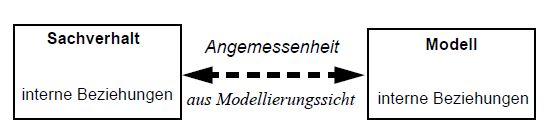
\includegraphics[scale=1]{Graphics/Sachverhalt.jpg}
		
		\captionof{figure}{Beziehung zwischen Modell und zu modellierendem Sachverhalt }
		
		
		Quelle : \cite{MT010}
		
		
		
		\label{fig9}
		
		
	\end{figure}
	
\end{center}

Modelle bedürfen immer der Überprüfung mit dem zu modellierenden Sachverhalt. Zwischen Sachverhalt
und Modell existiert immer eine Beziehung, die ein Maß für die Angemessenheit des Modells ist.
Die Bewertung der Angemessenheit eines Modells kann nur relativ zum Modellierungszweck erfolgen,
da Modelle von unwesentlichen Details abstrahieren. Im allgemeinen kann diese Beziehung nicht
direkt angeben werden, da der Sachverhalt meistens nur unklar spezifiziert ist. Aus diesem Grund ist
es auch nicht möglich, immer automatisch zu überprüfen, ob ein Modell den gewünschten Sachverhalt
modelliert. Nur wenn der Sachverhalt selbst als exakte Beschreibung vorliegt und auch das Modell
exakt beschrieben ist, wird ein formales Überprüfen erst möglich, und die Angemessenheit eines
Modells kann formal bewertet werden. Meistens ist der Sachverhalt jedoch nicht klar spezifiziert.
Die einzige Möglichkeit ist dann, den Inhalt des Modells zu erfassen und zu überprüfen, ob dieser mit
dem zu modellierenden Sachverhalt übereinstimmt. Je exakter und präziser ein Modell interpretiert
werden kann, desto leichter kann es mit dem zu modellierenden Sachverhalt verglichen werden.
Obwohl es nicht möglich ist, die Adäquanz zwischen einer eventuell unpräzisen Darstellung (Sachverhalt)
und einer möglichst präzisen Darstellung (Modell) prinzipiell zu entscheiden, hilft eine präzise
Darstellung und eindeutige Interpretation des Modells beim Vergleich mit dem zu modellierenden
Sachverhalt. Eine Modellierungssprache, die es ermöglicht, Modelle exakt und eindeutig zu beschreiben
und zu interpretieren, erleichtert daher wesentlich die Überprüfung des Modells.
Nur wenn Modelle eindeutig sind, ist eine korrekte Verständigung möglich. Dies verlangt eine eindeutige
Interpretation der einzelnen Sprachmittel und Regeln zur syntaktischen Verknüpfung dieser
Sprachmittel. Andernfalls bieten sich Interpretationsfreiräume, die zu Missverständnissen führen können.
Die exakte Festlegung der abstrakten Syntax und Semantik der Sprache ist somit Voraussetzung
für die eindeutige Interpretierbarkeit der Modelle. Beim Betrachten eines Artefakts der Modellierungssprache
hat man im allgemeinen nicht wie bei Programmen die Möglichkeit, durch Inspizieren oder
Ausprobieren des Codes die Aufgabe der Software herauszubekommen. Vielmehr ist die Beschreibung
der Metasprache die einzige Referenz.\\
Ein anderer Aspekt der Überprüfung betrifft die Nachvollziehbarkeit und Rückverfolgung von Modellierungsentscheidungen.\\\cite{MT010}
